%第4-2章
\section{検証}
ここから、4.1節で実装したプログラムの動作の検証と、他のメンバー担当箇所との統合後の、システム全体の動作の検証を行った。ここでも、V字モデルの開発プロセスに従い、単体テスト、結合テスト、総合テストという順番で検証を行っている。

\subsection{単体テスト}
まずはじめに、実装の段階で検証が求められるレベルの項目について、単体テストを行った。ここでは、実装担当者が中心となって、各担当箇所の検証項目について検証を行った。以下に、私の担当箇所に関する単体テストの内容について述べる。

ここでは、Jetson nano側でのシステム全体の制御に関する部分と、データベース操作に関する部分それぞれについて単体テストを行った。まず、Jetson nano側でのシステム全体の制御に関する部分の単体テストを表\ref{jtantaitest}に示す。

\begin{table}[H]
	\centering
	\caption{jetson nano単体テスト}
	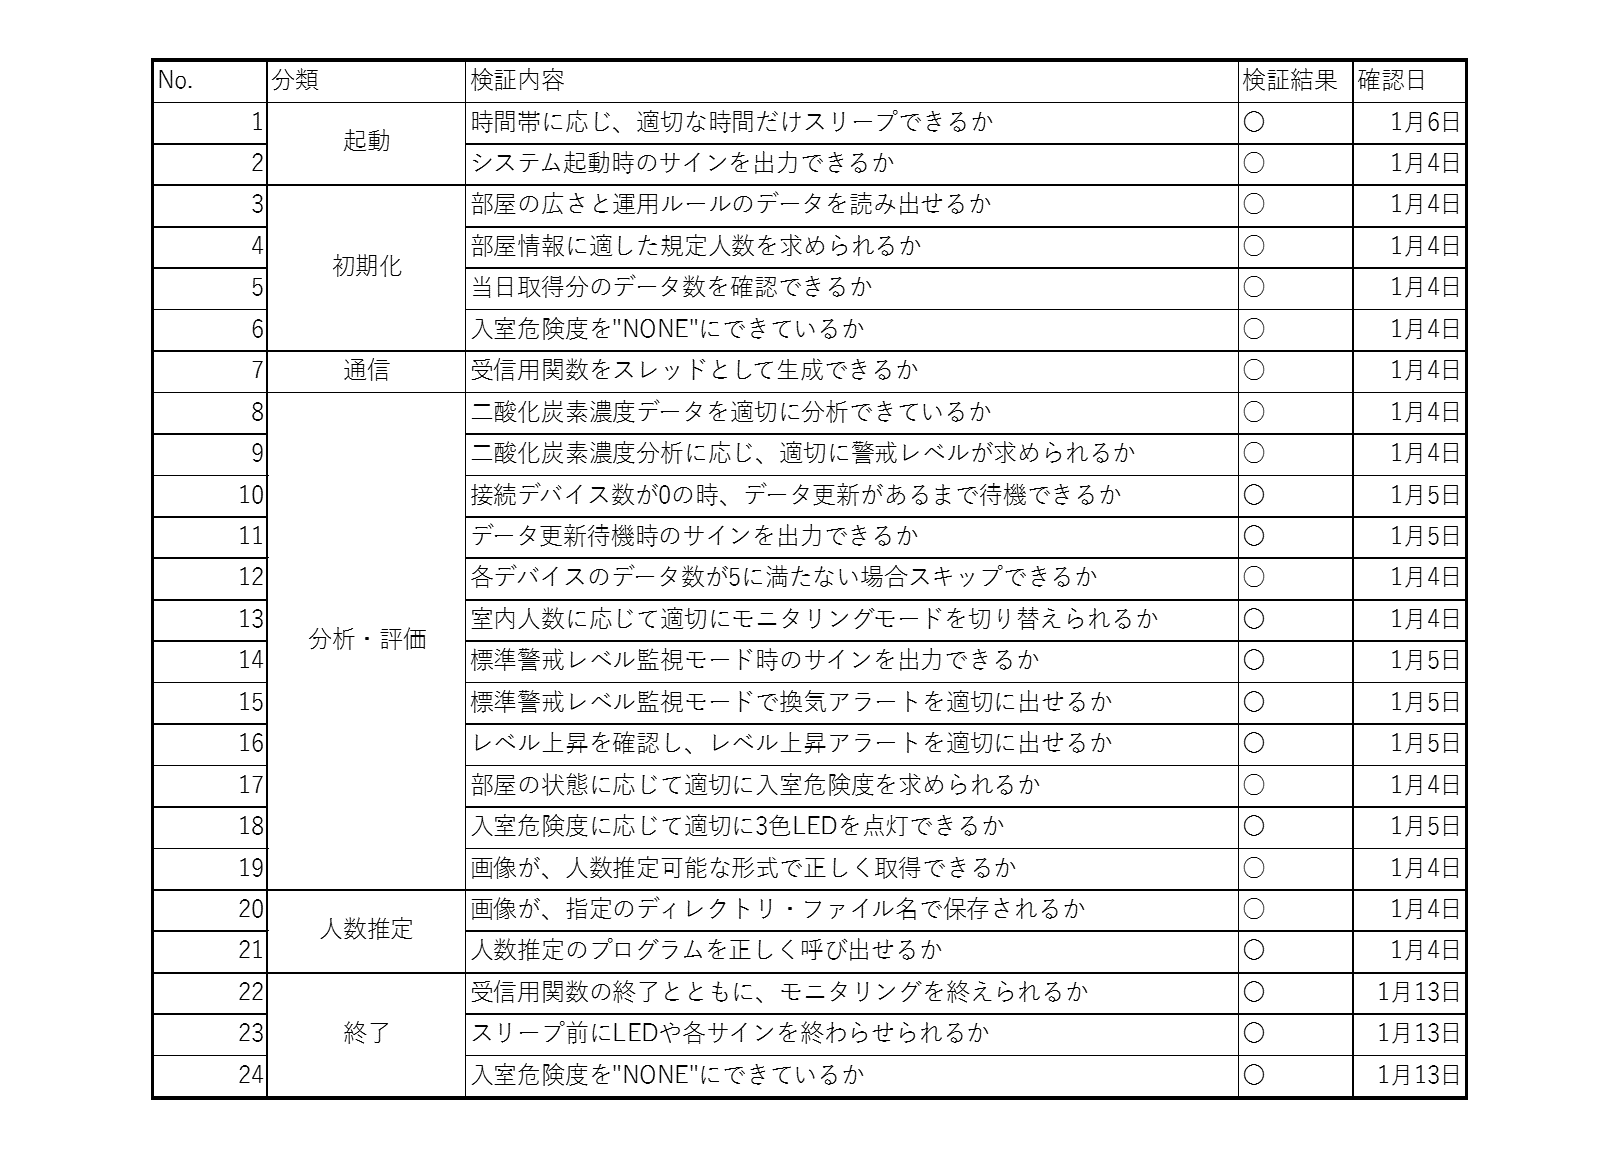
\includegraphics[width=15cm]{jtantaitest.eps}
	\label{jtantaitest}
\end{table}

jetson nano側でデータベース操作以外で実行するのは、4.1節で説明したメインプログラムと各デバイスとの通信用プログラムである。ここではこれらプログラムのうち、メソッドなどの比較的細かな単位で検証を行った。実際のシステム運用時には、他のデバイスとの通信やデータベースの操作などが関わってくるが、手作業で値を与えるなど、疑似的に動作環境をつくり動作を確認した。

ここで特に問題となったのは、LEDを用いた各種サインの出力に関する部分で、それぞれをメインプログラムとは別のスレッドとして生成させて実行するが、状況によっては複数スレッドが同時にGPIOに対し操作してしまう状況があることに気づいた。そのためLEDによるサインを、システム内部の処理によって本来切り替えるべきタイミングで即時切り替えるのではなく、GPIOを操作するスレッドを正常に停止できるまで、GPIOを操作する別スレッドの生成を待機させることでGPIOの操作の一時的な衝突を回避するという修正が必要となった。

続いて、データベース操作に関する部分の単体テストを表\ref{dtantaitest}に示す。

\begin{table}[H]
	\centering
	\caption{データベース単体テスト}
	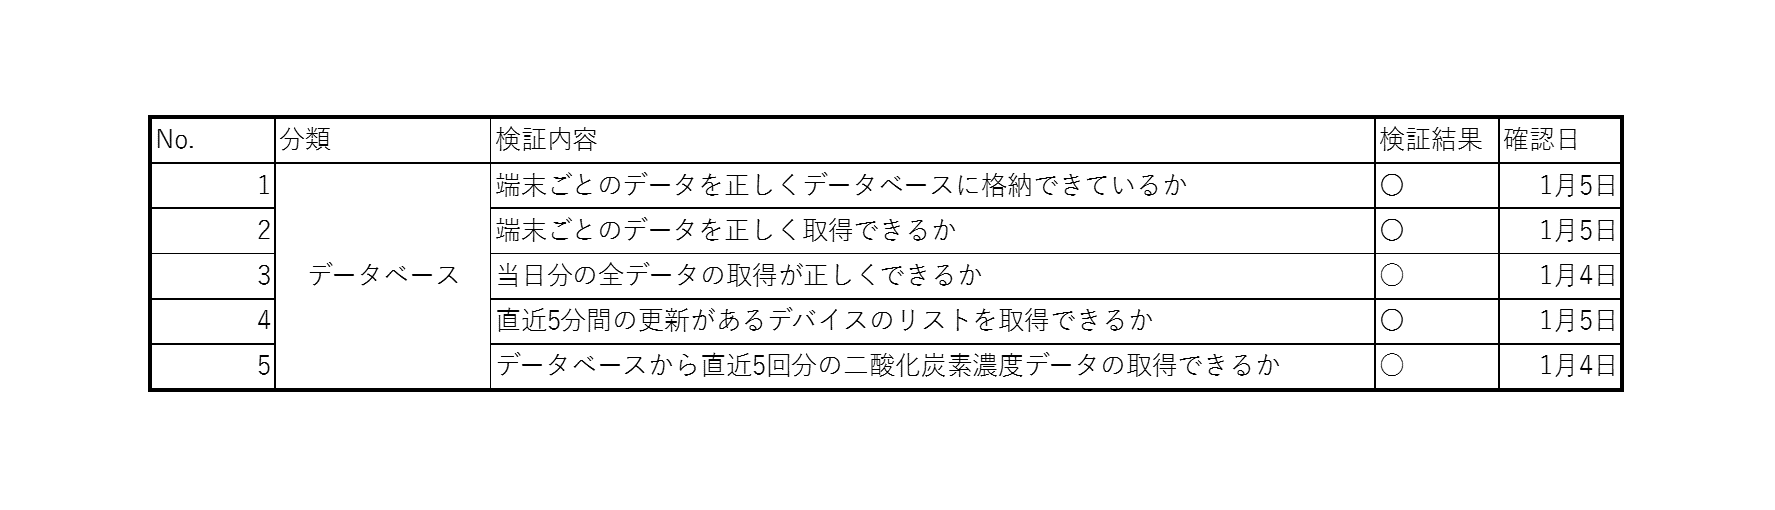
\includegraphics[width=15cm]{dtantaitest.eps}
	\label{dtantaitest}
\end{table}

ここでは、センサデバイスからの取得データに対するデータベースの動作を検証するかわりに、疑似的なデータを与えた場合に、想定した操作を行えるかどうかを検証したが、概ね問題なく動作することが確認できた。

\subsection{結合テスト}
結合テストでは、Jetson nano側で動作するメインプログラムと、データベース操作のプログラムの連携のほか、他のメンバーの担当箇所との統合も含めてテストを行い、デバイス類との通信に関する部分や、人数推定プログラムの動作も検証した。ここで、実施した結合テストを表\ref{ketugoutest}に示す。

\begin{table}[H]
	\centering
	\caption{結合テスト}
	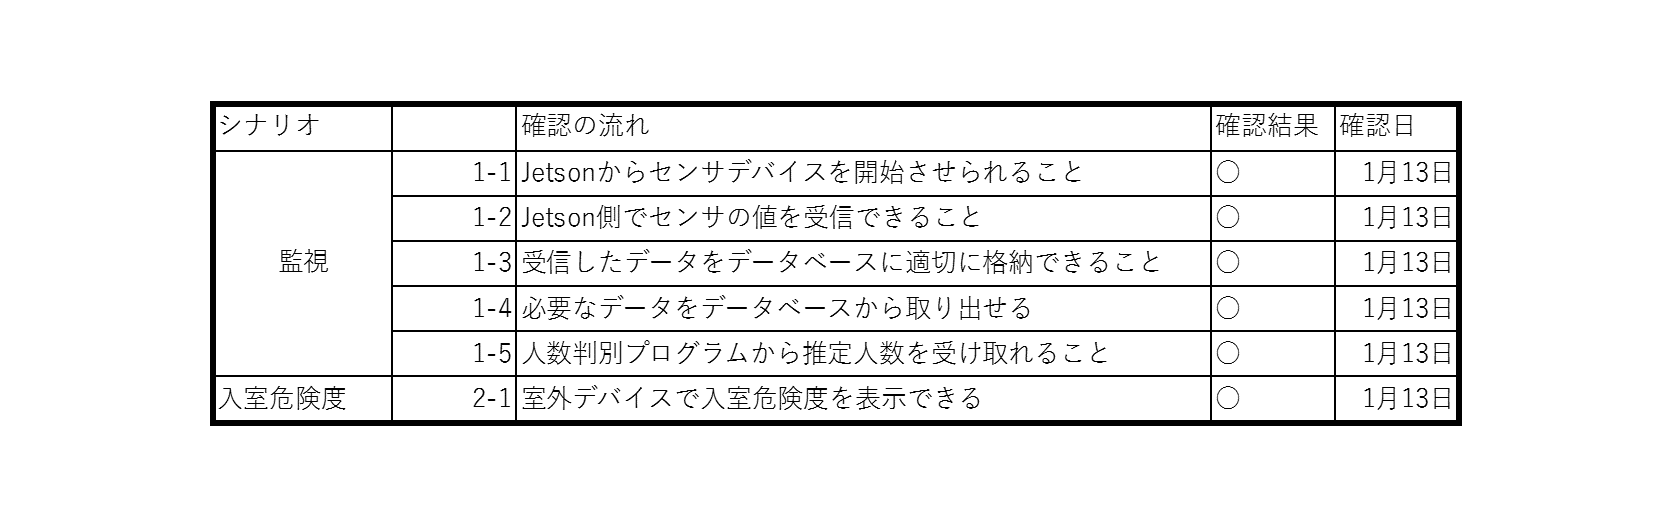
\includegraphics[width=15cm]{ketugoutest.eps}
	\label{ketugoutest}
\end{table}

結合テスト実施までに、各自の担当箇所について単体テストを実施し、プログラムやメソッド、関数等が単体で正常に動作することが確認された。結合テストでは、単体テストの検証項目について、動作が保証されたうえで、それらを組み合わせた場合の動作を確認できた。


\subsection{総合テスト}
総合テストでは、実際の運用を想定した環境で検証を行った。ただし、感染症予防の観点から大人数を集めて、二酸化炭素濃度の変動を確認したり、人数推定プログラムで何十人という人の数をどれくらいの精度で確認できるかといったことまでは、今回は確認することができていない。ここで、実施した総合テストを表\ref{sougoutest}に示す。

\begin{table}[H]
	\centering
	\caption{総合テスト}
	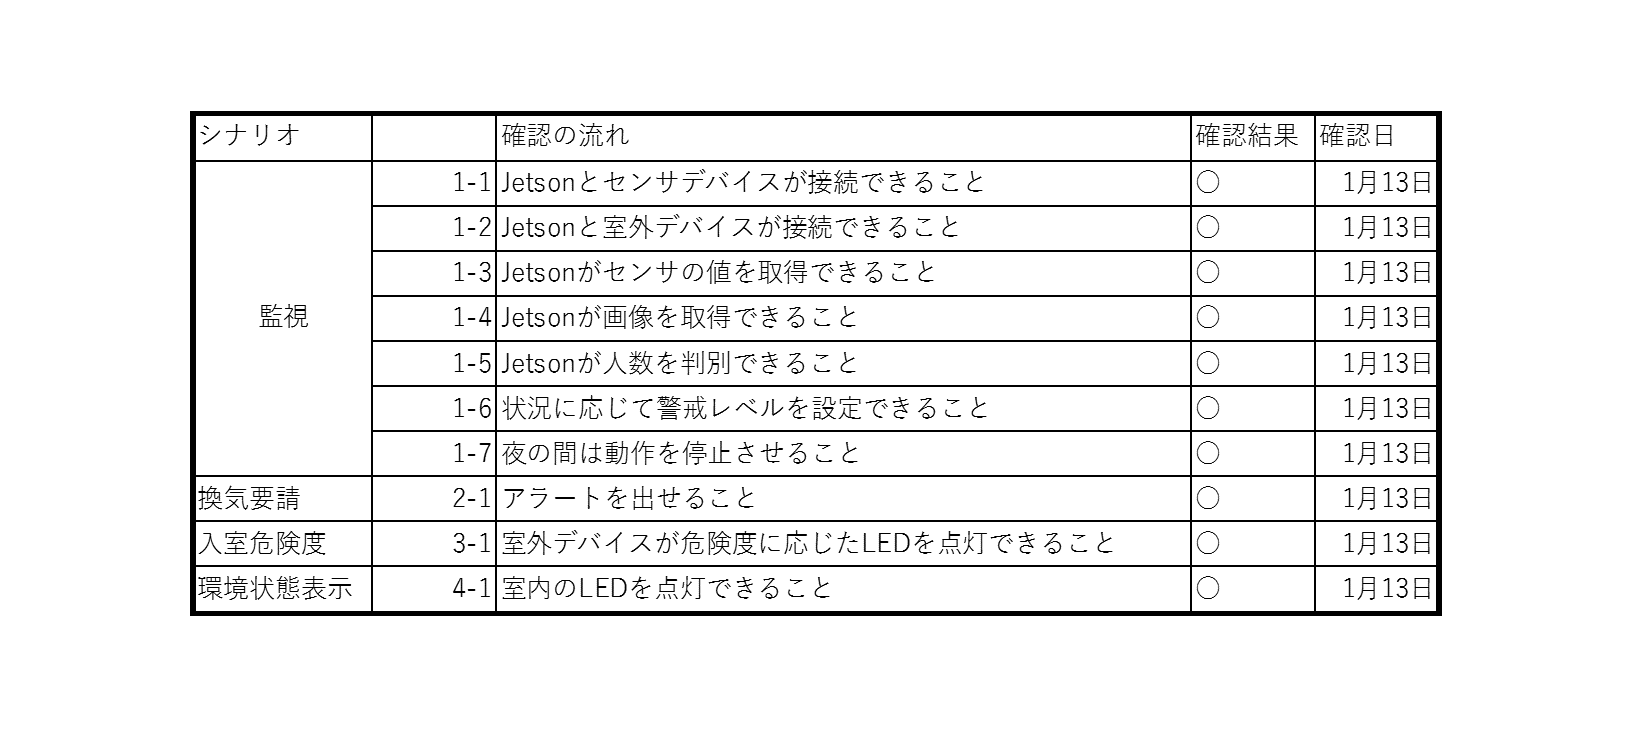
\includegraphics[width=15cm]{sougoutest.eps}
	\label{sougoutest}
\end{table}

このように、最終的に4つのユースケースを満足できることを確認するために、実際のシステム利用環境で検証を行い、各自の担当箇所がうまく統合され、正しく動作することを確認した。

また、デバイス類との接続とデータの取得・管理が正しく動作することを、結合・総合テストの実施によって確認できたことを踏まえ、部屋の滞在人数や換気状況の変化に対するシステムの動作確認を行うために、室内環境を仮想的に表すデータとして、表4.6のようなデータを3分ごとにデータベースに与えて動作させた。なお、表4.6はテストデータを記録したデータベースの内容を示しており、recordIDはレコードに割り当てられた通し番号、dtはセンサデータ取得日時、devIDはセンサデータを送ったデバイスのID、co2が二酸化炭素濃度を示す。以下のデータは、センサデバイス2台の3分おき20回分のデータ取得を想定している。ただし実際には、このほかにもいくつかのフィールドがデータベースに記録されているが、ここでは省略している。


\begin{longtable}{|c|c|c|c|}
	\caption{テストデータ}
	\label{testdata}
	\endhead
	\hline
	recordID & dt & devID & co2\\ \hline \hline
	1 & 2021-01-16 14:38:43 & 1 & 581\\
	2 & 2021-01-16 14:38:43 & 2 & 580\\
	3 & 2021-01-16 14:41:43 & 1 & 587\\
	4 & 2021-01-16 14:41:43 & 2 & 592\\
	5 & 2021-01-16 14:44:43 & 1 & 593\\
	6 & 2021-01-16 14:44:43 & 2 & 603\\ 
	7 & 2021-01-16 14:47:43 & 1 & 622\\ 
	8 & 2021-01-16 14:47:43 & 2 & 621\\ 
	9 & 2021-01-16 14:50:43 & 1 & 644\\ 
	10 & 2021-01-16 14:50:43 & 2 & 656\\ 
	11 & 2021-01-16 14:53:43 & 1 & 667\\ 
	12 & 2021-01-16 14:53:43 & 2 & 694\\
	13 & 2021-01-16 14:56:43 & 1 & 689\\
	14 & 2021-01-16 14:56:43 & 2 & 712\\ 
	15 & 2021-01-16 14:59:43 & 1 & 703\\
	16 & 2021-01-16 14:59:43 & 2 & 739\\
	17 & 2021-01-16 15:02:43 & 1 & 724\\
	18 & 2021-01-16 15:02:43 & 2 & 802\\
	19 & 2021-01-16 15:05:43 & 1 & 769\\
	20 & 2021-01-16 15:05:43 & 2 & 812\\
	21 & 2021-01-16 15:08:43 & 1 & 796\\
	22 & 2021-01-16 15:08:43 & 2 & 833\\
	23 & 2021-01-16 15:11:43 & 1 & 811\\
	24 & 2021-01-16 15:11:43 & 2 & 855\\
	25 & 2021-01-16 15:14:43 & 1 & 824\\
	26 & 2021-01-16 15:14:43 & 2 & 889\\
	27 & 2021-01-16 15:17:43 & 1 & 829\\
	28 & 2021-01-16 15:17:43 & 2 & 856\\
	29 & 2021-01-16 15:20:43 & 1 & 811\\
	30 & 2021-01-16 15:20:43 & 2 & 833\\ 
	31 & 2021-01-16 15:23:43 & 1 & 798\\
	32 & 2021-01-16 15:23:43 & 2 & 791\\
	33 & 2021-01-16 15:26:43 & 1 & 783\\ 
	34 & 2021-01-16 15:26:43 & 2 & 786\\ 
	35 & 2021-01-16 15:29:43 & 1 & 779\\
	36 & 2021-01-16 15:29:43 & 2 & 784\\ 
	37 & 2021-01-16 15:32:43 & 1 & 753\\
	38 & 2021-01-16 15:32:43 & 2 & 779\\
	39 & 2021-01-16 15:35:43 & 1 & 737\\ 
	40 & 2021-01-16 15:35:43 & 2 & 771\\ \hline
\end{longtable}

また、上のデータを与えた場合に求められる、室内の二酸化炭素濃度代表値と警戒レベルは以下のようになり、滞在人数の値に対して、感染リスクが求められる様子を確認した。ただし、システムの運用環境は、広さが100平方メートルで、5平方メートルに1人までが滞在でき、最大で20人までが滞在可能な部屋を想定している。

\begin{longtable}{|c|c|c|c|c|c|}
\caption{分析結果と滞在人数に対するリスク評価}
\label{testresult}
\endhead
\hline
番号 & 日時 & co2代表値 & 警戒レベル & 滞在人数 & 感染リスク\\ \hline \hline
1 & 2021-01-16 14:38:43 & - & 0 & 8 & -\\
2 & 2021-01-16 14:41:43 & - & 0 & 9 & -\\
3 & 2021-01-16 14:44:43 & - & 0 & 8 & -\\
4 & 2021-01-16 14:47:43 & - & 0 & 10 & -\\ 
5 & 2021-01-16 14:50:43 & 581 & 0 & 14 & -\\ 
6 & 2021-01-16 14:53:43 & 592 & 1 & 15 & green\\ 
7 & 2021-01-16 14:56:43 & 603 & 1 & 15 & green\\
8 & 2021-01-16 14:59:43 & 622 & 1 & 17 & green\\
9 & 2021-01-16 15:02:43 & 656 & 1 & 16 & green\\
10 & 2021-01-16 15:05:43 & 694 & 1 & 17 & green\\
11 & 2021-01-16 15:08:43 & 712 & 2 & 17 & green\\
12 & 2021-01-16 15:11:43 & 739 & 2 & 18 & yellow\\
13 & 2021-01-16 15:14:43 & 802 & 3 & 18 & red\\
14 & 2021-01-16 15:17:43 & 812 & 3 & 17 & yellow\\
15 & 2021-01-16 15:20:43 & 833 & 3 & 16 & green\\
16 & 2021-01-16 15:23:43 & 798 & 2 & 15 & green\\
17 & 2021-01-16 15:26:43 & 786 & 2 & 15 & green\\ 
18 & 2021-01-16 15:29:43 & 784 & 2 & 16 & green\\
19 & 2021-01-16 15:32:43 & 779 & 2 & 17 & green\\
20 & 2021-01-16 15:35:43 & 771 & 2 & 18 & yellow\\ \hline
\end{longtable}

以上のデータは、室内にほとんど人がいない状態から徐々に人数が増えていき、二酸化炭素濃度・警戒レベルが上昇し、換気アラートが出され、感染リスクが高まったことを受け、換気が行われ感染リスクが安全水準に戻される様子を想定している。

今回は、初回起動時を想定したため、データの始まりは14時台であるものの二酸化炭素濃度分析のために必要な5回分の取得データがない状態から始まり、警戒レベルは初めに0に設定され、初めの4回分のデータ分析では、部屋の二酸化炭素濃度の代表値は導出されない。このように、データ数が少ない時には、提供できる情報がないものの、システムが稼働していることは利用者に知らせる必要があることから、スタンバイ中であることを示すLEDサインを出力する。また、数分前に感染リスク評価を行っていた場合でも、接続デバイスから長時間データ更新がされなかった場合には、その感染リスクの情報の信憑性が下がることから、同じサインを出力させることとなっている。

5回目以降の分析時には、分析に必要なデータ数が揃ったことで、部屋の二酸化炭素濃度の代表値が定められ、警戒レベルと感染リスクの評価が行われる。ただし、5回目の分析では、室内の滞在人数が20人の75\%を下回るため、警戒レベルとリスクの評価は行われない。

以降のデータ分析に関しても、上で示したテストデータと室内人数から、設計通りの分析ができたことが確認でき、二酸化炭素濃度の上昇に伴って、滞在可能な人数が制限され、より少ない人数しか滞在していない場合でも感染リスクが厳しくつけられ、警戒レベル上昇時に出される換気要請とともに、利用者に対して感染予防のためのアクションを促す機能が、設計通り実現されていることが確認できた。

今回は二酸化炭素濃度や室内の人数の変動を、実際の利用環境で再現することを避けたことから、このようなテスト環境で検証を行うこととなった。実際の利用環境でのテスト稼働時にも、授業などで大人数が出入りし、二酸化炭素濃度が上昇し警戒レベルを高めるような、実際の運用時に想定される環境変化こそ再現できていないものの、実際のシステム利用環境であっても、仮想的な室内環境を想定し、疑似的なデータを与えた検証時と同じように、設計通りの動作ができることが確認された。



